\chapter{Planificación y Diseño.} \label{ch:planificacion_disenio}

\section{Planificación.} \label{sec:planificacion}

En un proyecto de estas dimensiones la planificación es fundamental. La planificación que he seguido la podemos ver en el siguiente diagrama de Gannt:

\begin{figure}[ht]
\begin{ganttchart}[
  canvas/.append style={fill=none, draw=black!5, line width=.75pt},
  vgrid={*1{draw=black!5, line width=.75pt}},
  today=20,
  today label font=\scriptsize\scshape,
  title/.style={draw=none, fill=none},
  title label font=\scshape\footnotesize,
  title label node/.append style={below=7pt},
  include title in canvas=false,
  bar/.append style={draw=none, fill=black!63}
  ]{1}{20}
  \gantttitlelist{"Sep", "Oct", "Nov", "Dic", "Ene", "Feb", "Mar", "Abr", "May", "Jun"}{2} \\
  \ganttbar{Investigación}{1}{3} \\
  \ganttbar{Análisis}{4}{5} \\
  \ganttbar{Diseño}{6}{7} \\
  \ganttbar{Implementación}{8}{17} \\
  \ganttbar{Pruebas}{10}{17} \\
  \ganttbar{Memoria}{16}{20}
\end{ganttchart}
\caption{Planificación del proyecto}
\label{fig:gantt}
\end{figure}

La planificación era bastante directa; las primeras semanas de investigación, para adquirir el conocimiento necesario para poder desarrollar este proyecto. A continuación, dado que es una biblioteca de gran tamaño, un mes de trabajo desarrollando diagramas de clases y analizando las mejores opciones para implementar los algoritmos. Finalmente, la parte más dura, implementar los algoritmos. Primero empecé implementando las estructuras de datos y funciones auxiliares que iba a necesitar para posteriormente facilitar la implementación de los algoritmos en sí. Desde que implementé el primero, comenzaron las pruebas para ver que los algoritmos eran correctos. Cuando se acercaba la etapa final del proyecto comencé con la memoria para no quedarme sin tiempo. 

\section{Diseño.} \label{sec:disenio}

Para poder agrupar las clases diseñadas según su funcionalidad se han creado los siguientes paquetes: 

\begin{itemize}
	\item \textit{core:} paquete principal de la biblioteca. Se usa para contener las clases asociadas a todos los algoritmos implementados.
	\item \textit{data:} paquete usado para contener todas las estructuras de datos e información usada por los algoritmos.
	\item \textit{io:} paquete usado para contener todas las clases destinadas a entrada y salida de datos.
	\item \textit{util:} paquete usado para contener una clase de utilidades, es decir, funciones usadas por varios algoritmos.
\end{itemize}

Todos los paquetes nombrados anteriormente se ubican dentro del paquete \textit{undersampling}. El diagrama de paquetes asociado a la biblioteca lo podemos ver a continuación:

\begin{figure}[H]
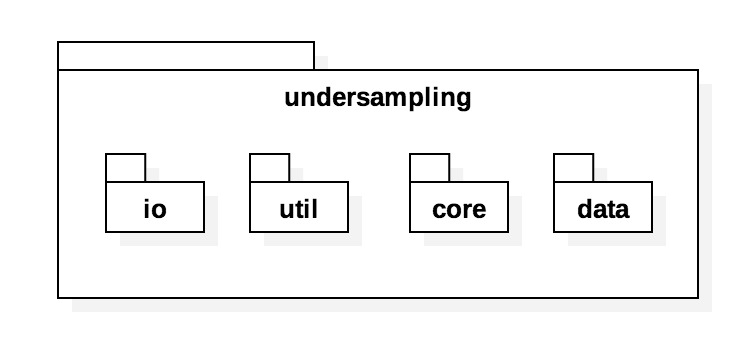
\includegraphics[width=0.80\linewidth]{./imagenes/3_paquetes.jpg}
\end{figure}

Tras diseñar los paquetes a usar, diseñé las clases que iba a necesitar para el proyecto. La estructura es bastante sencilla. Los algoritmos están implementados cada uno en su clase y todas ellas heredan de \textit{Algorithm}. Los algoritmos usan algunas funciones definidas en la clase \textit{Utilities} y usan un valor del enumerado \textit{Distances} para indicar la distancia a usar. Todos los algoritmos hacen uso de la estructura de datos representada por la clase \textit{Data}. A continuación podemos ver el diagrama de clases implementado:

\begin{figure}[H]
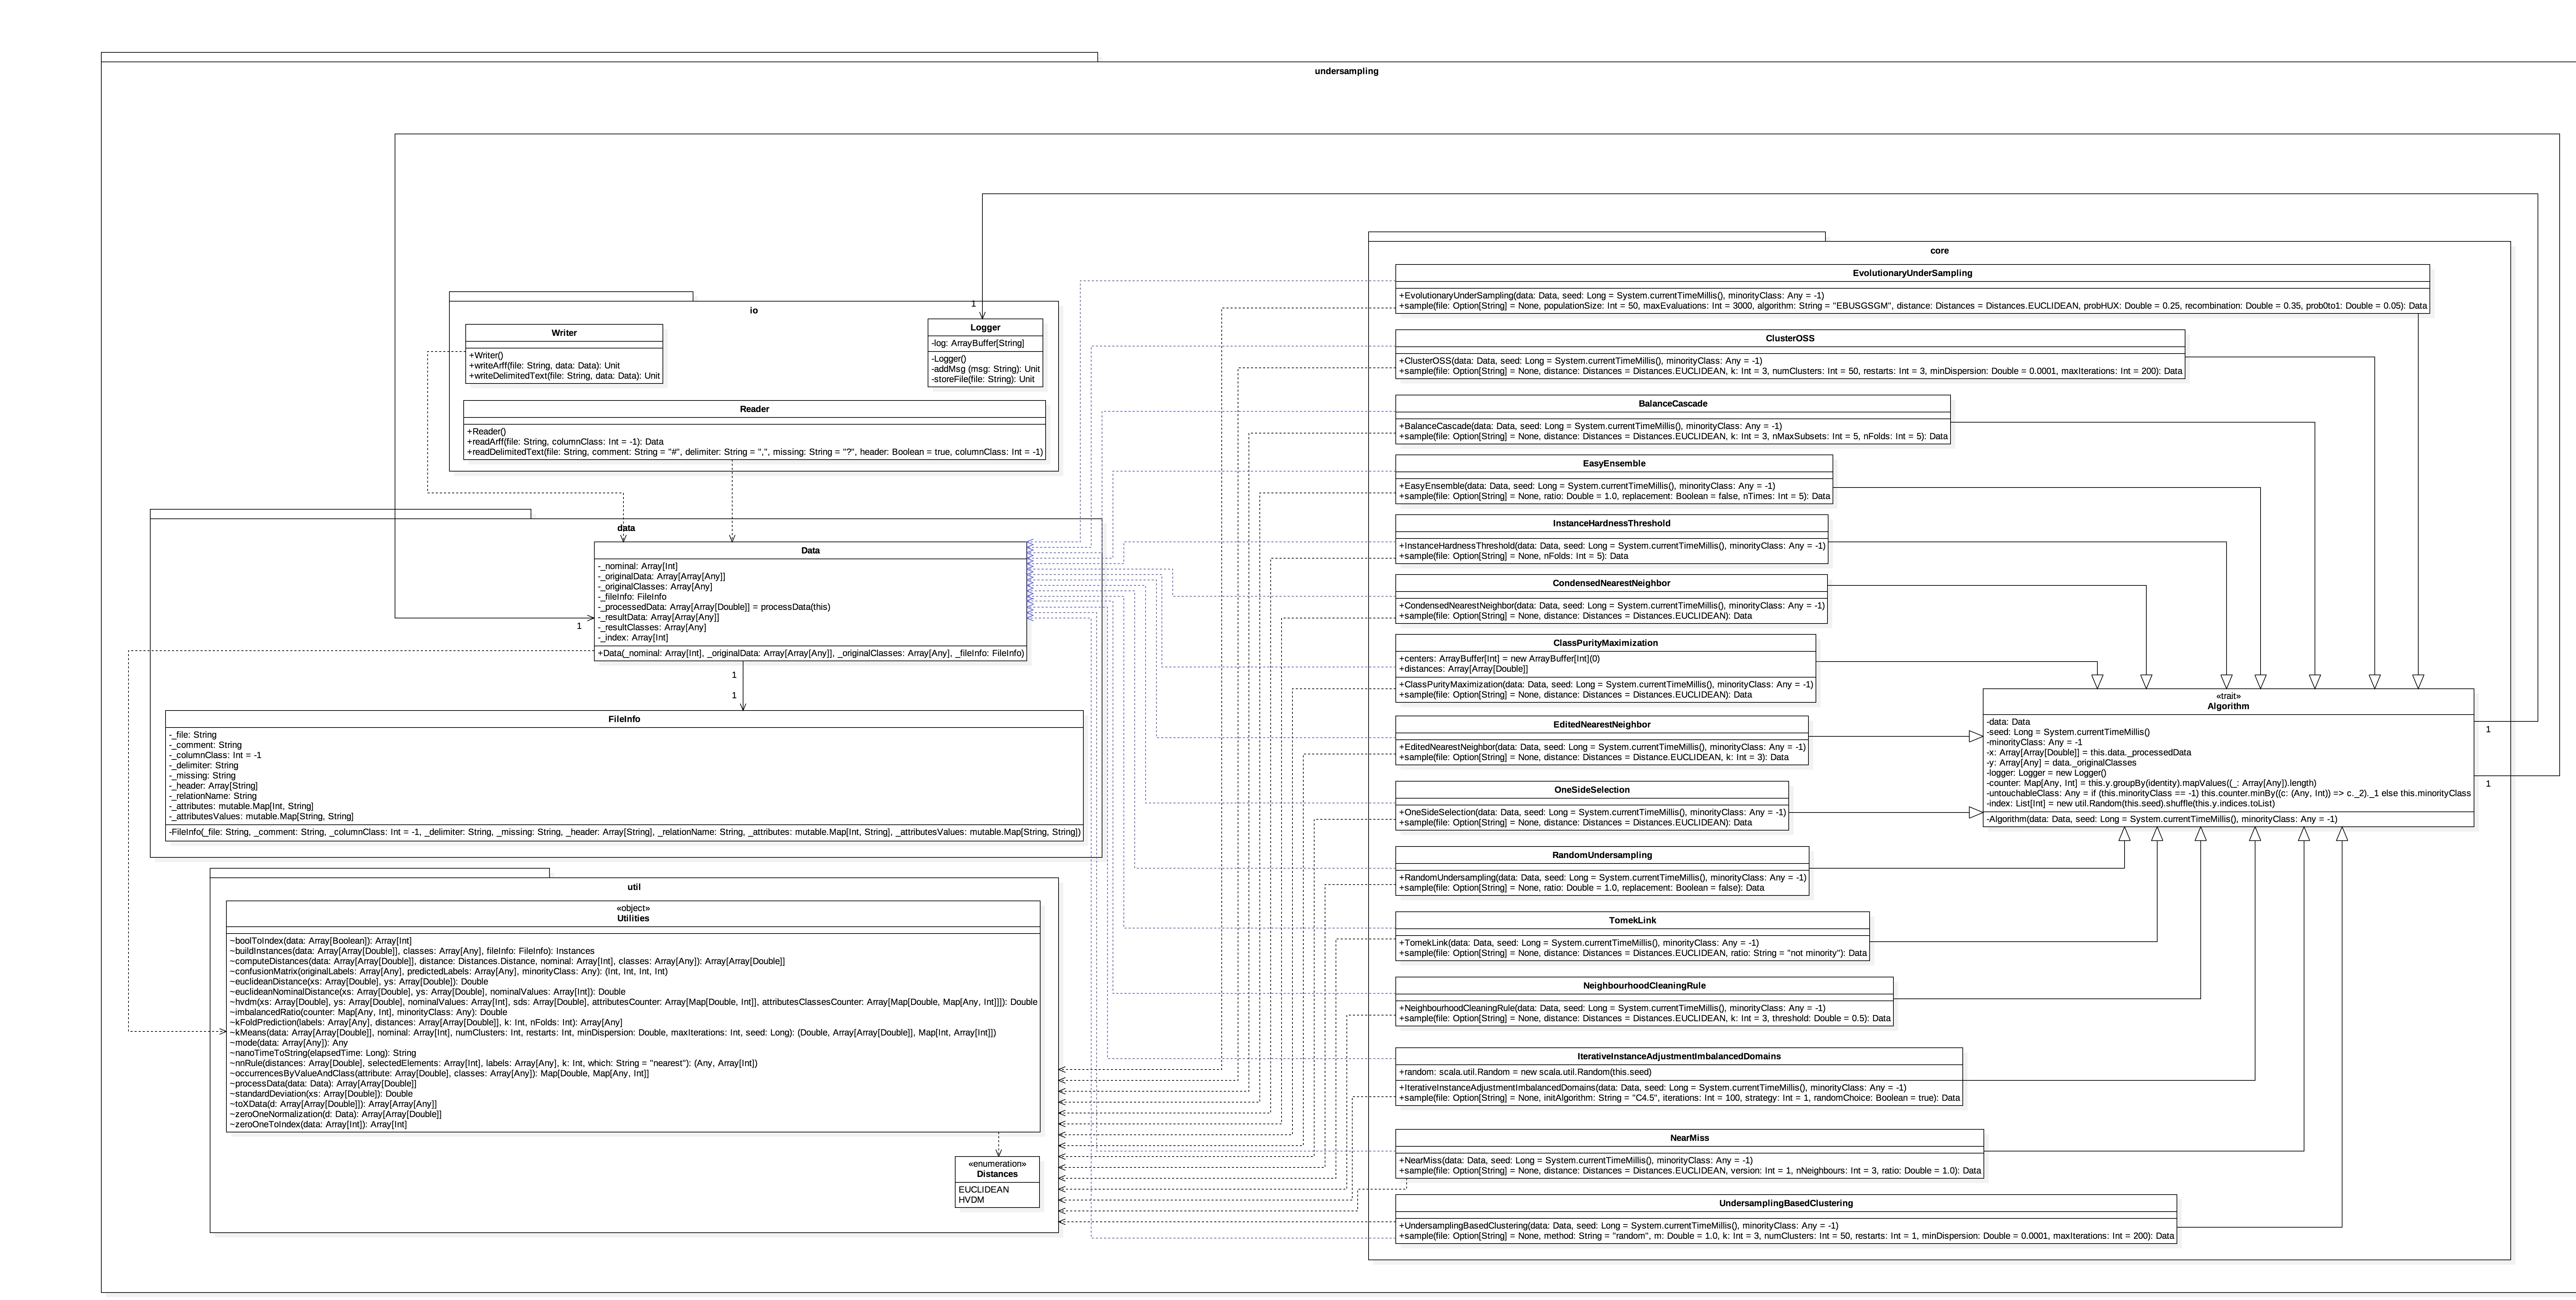
\includegraphics[scale=0.08, angle=90]{./imagenes/3_clases.jpg}
\end{figure}

Dado que no se puede ver con claridad cada clase, en la siguiente figura podemos ver un diagrama de clases simplificado, es decir, sin los métodos ni atributos de cada clase:

\begin{figure}[H]
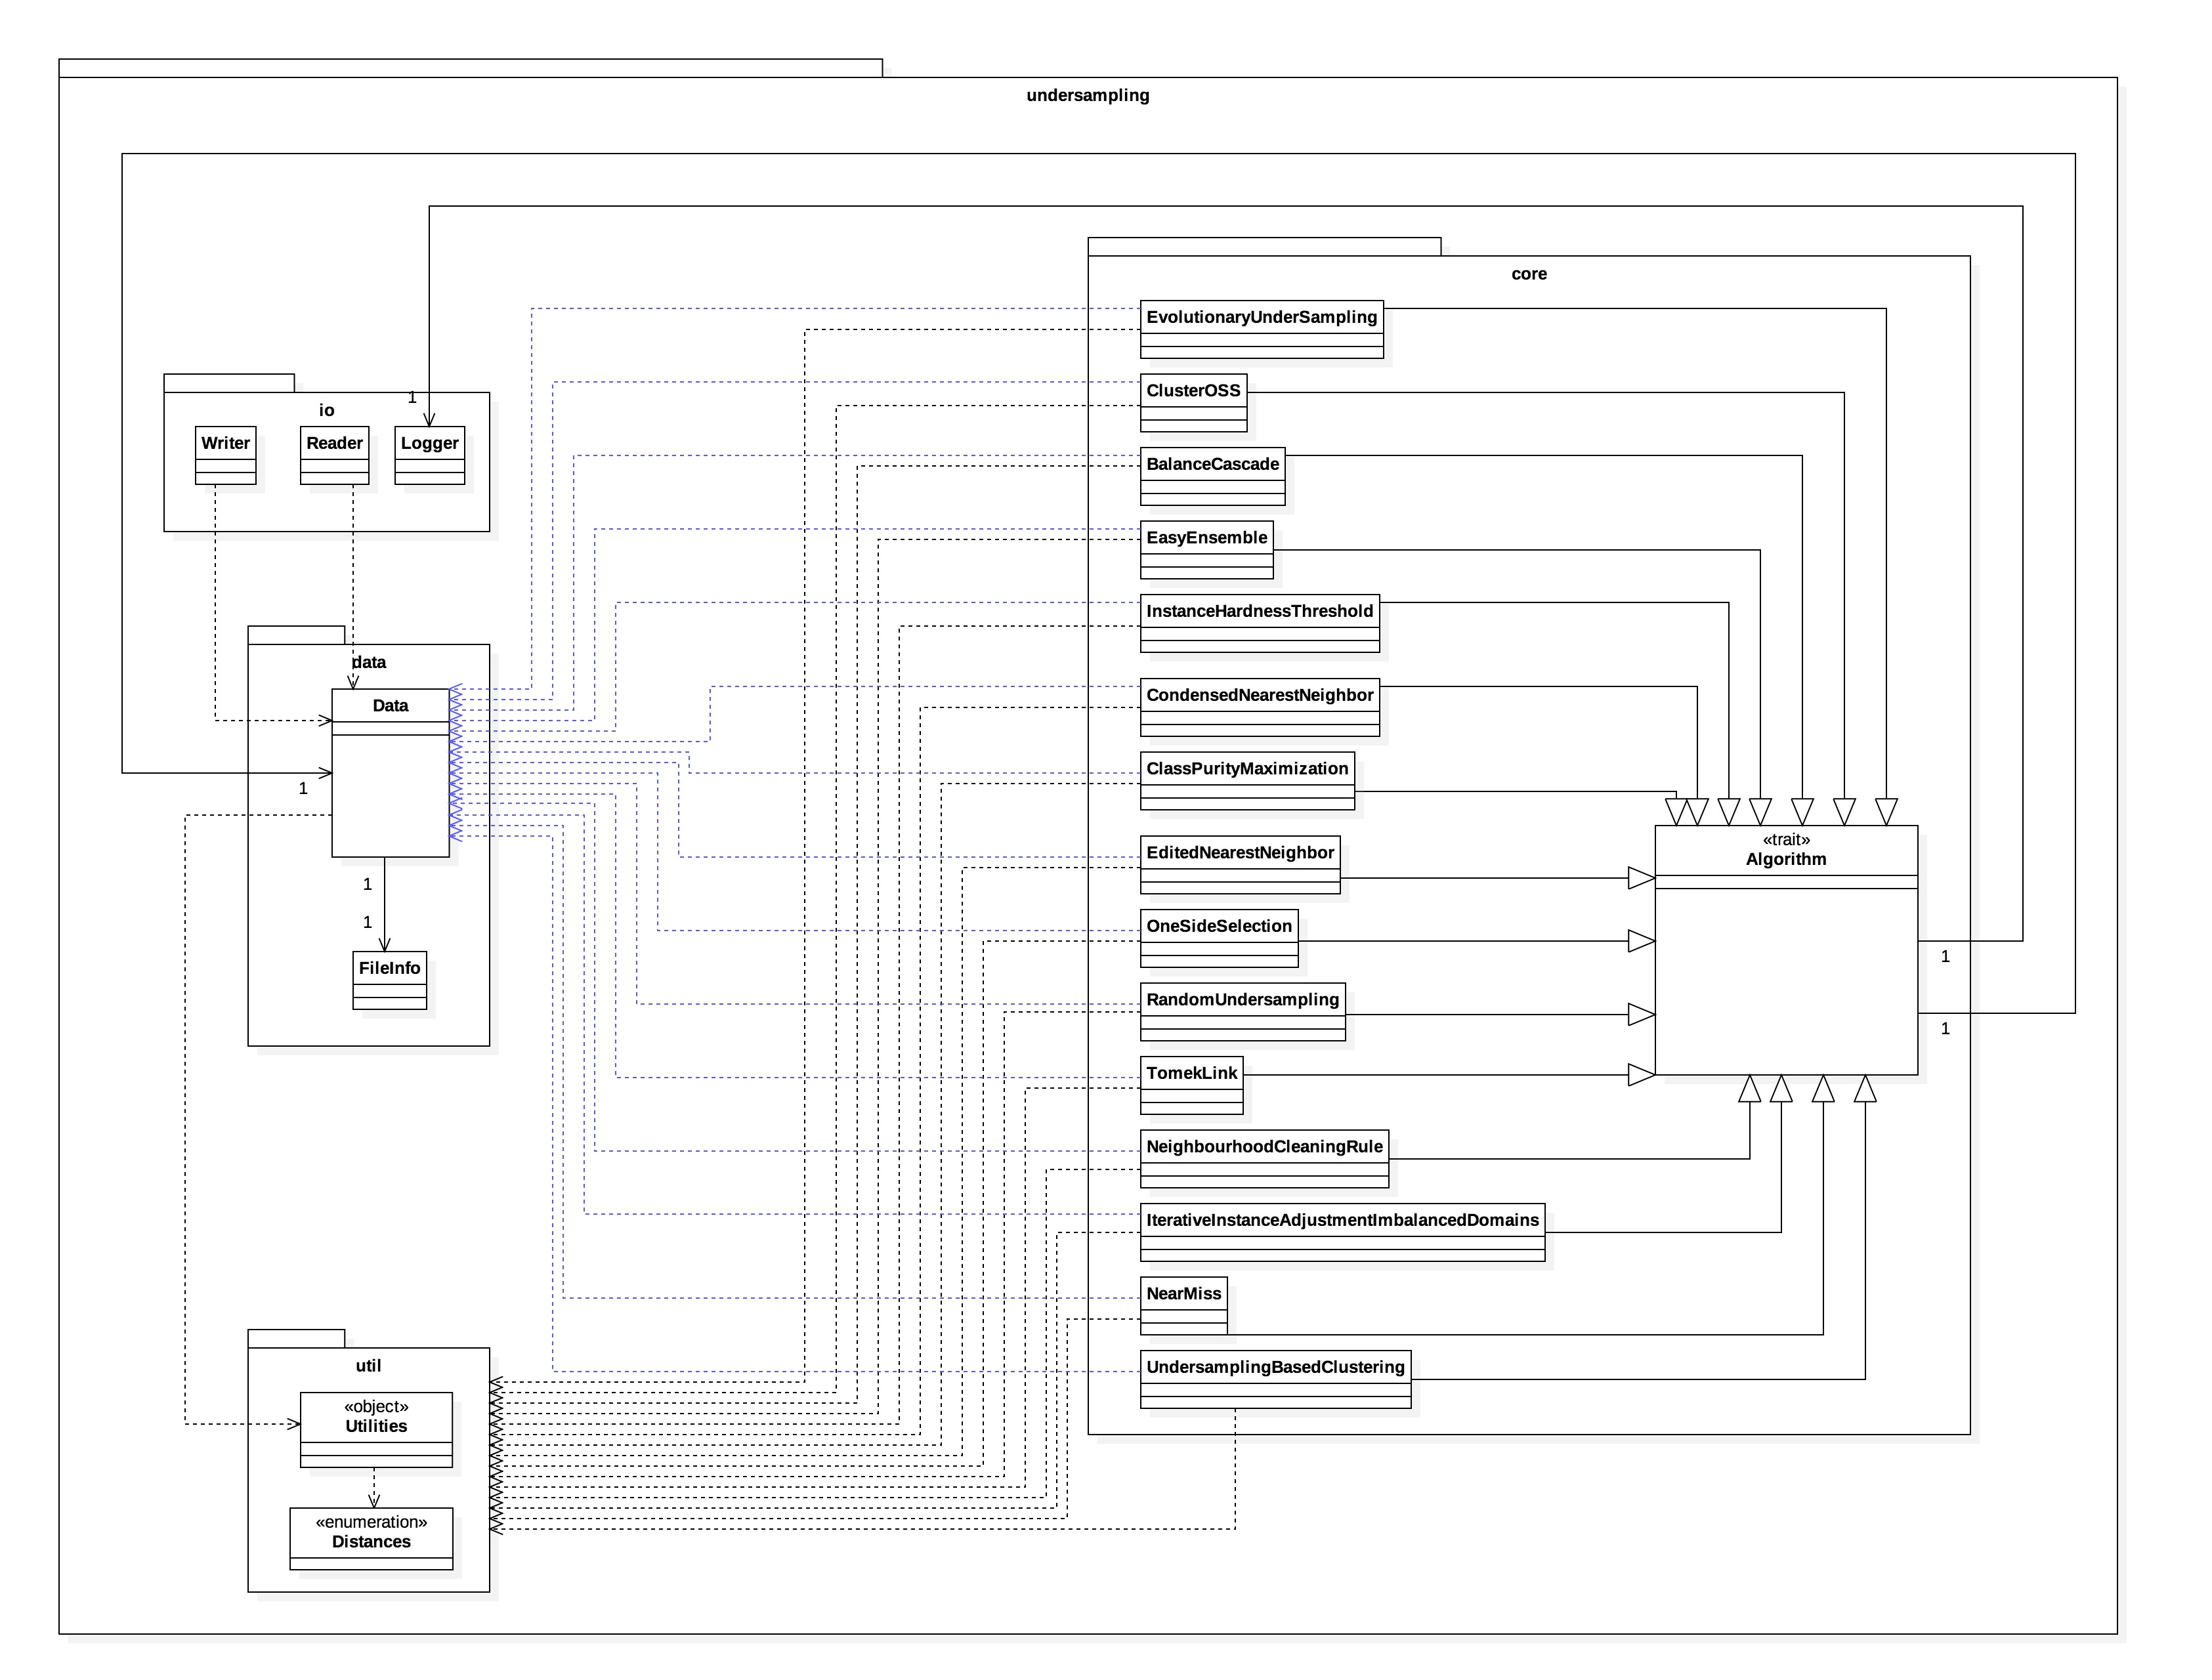
\includegraphics[scale=0.14, angle=90]{./imagenes/3_clases_simplificado.jpg}
\end{figure}

Para poder apreciar los detalles de cada clase, podemos ver las siguientes figuras:

\begin{figure}[H]
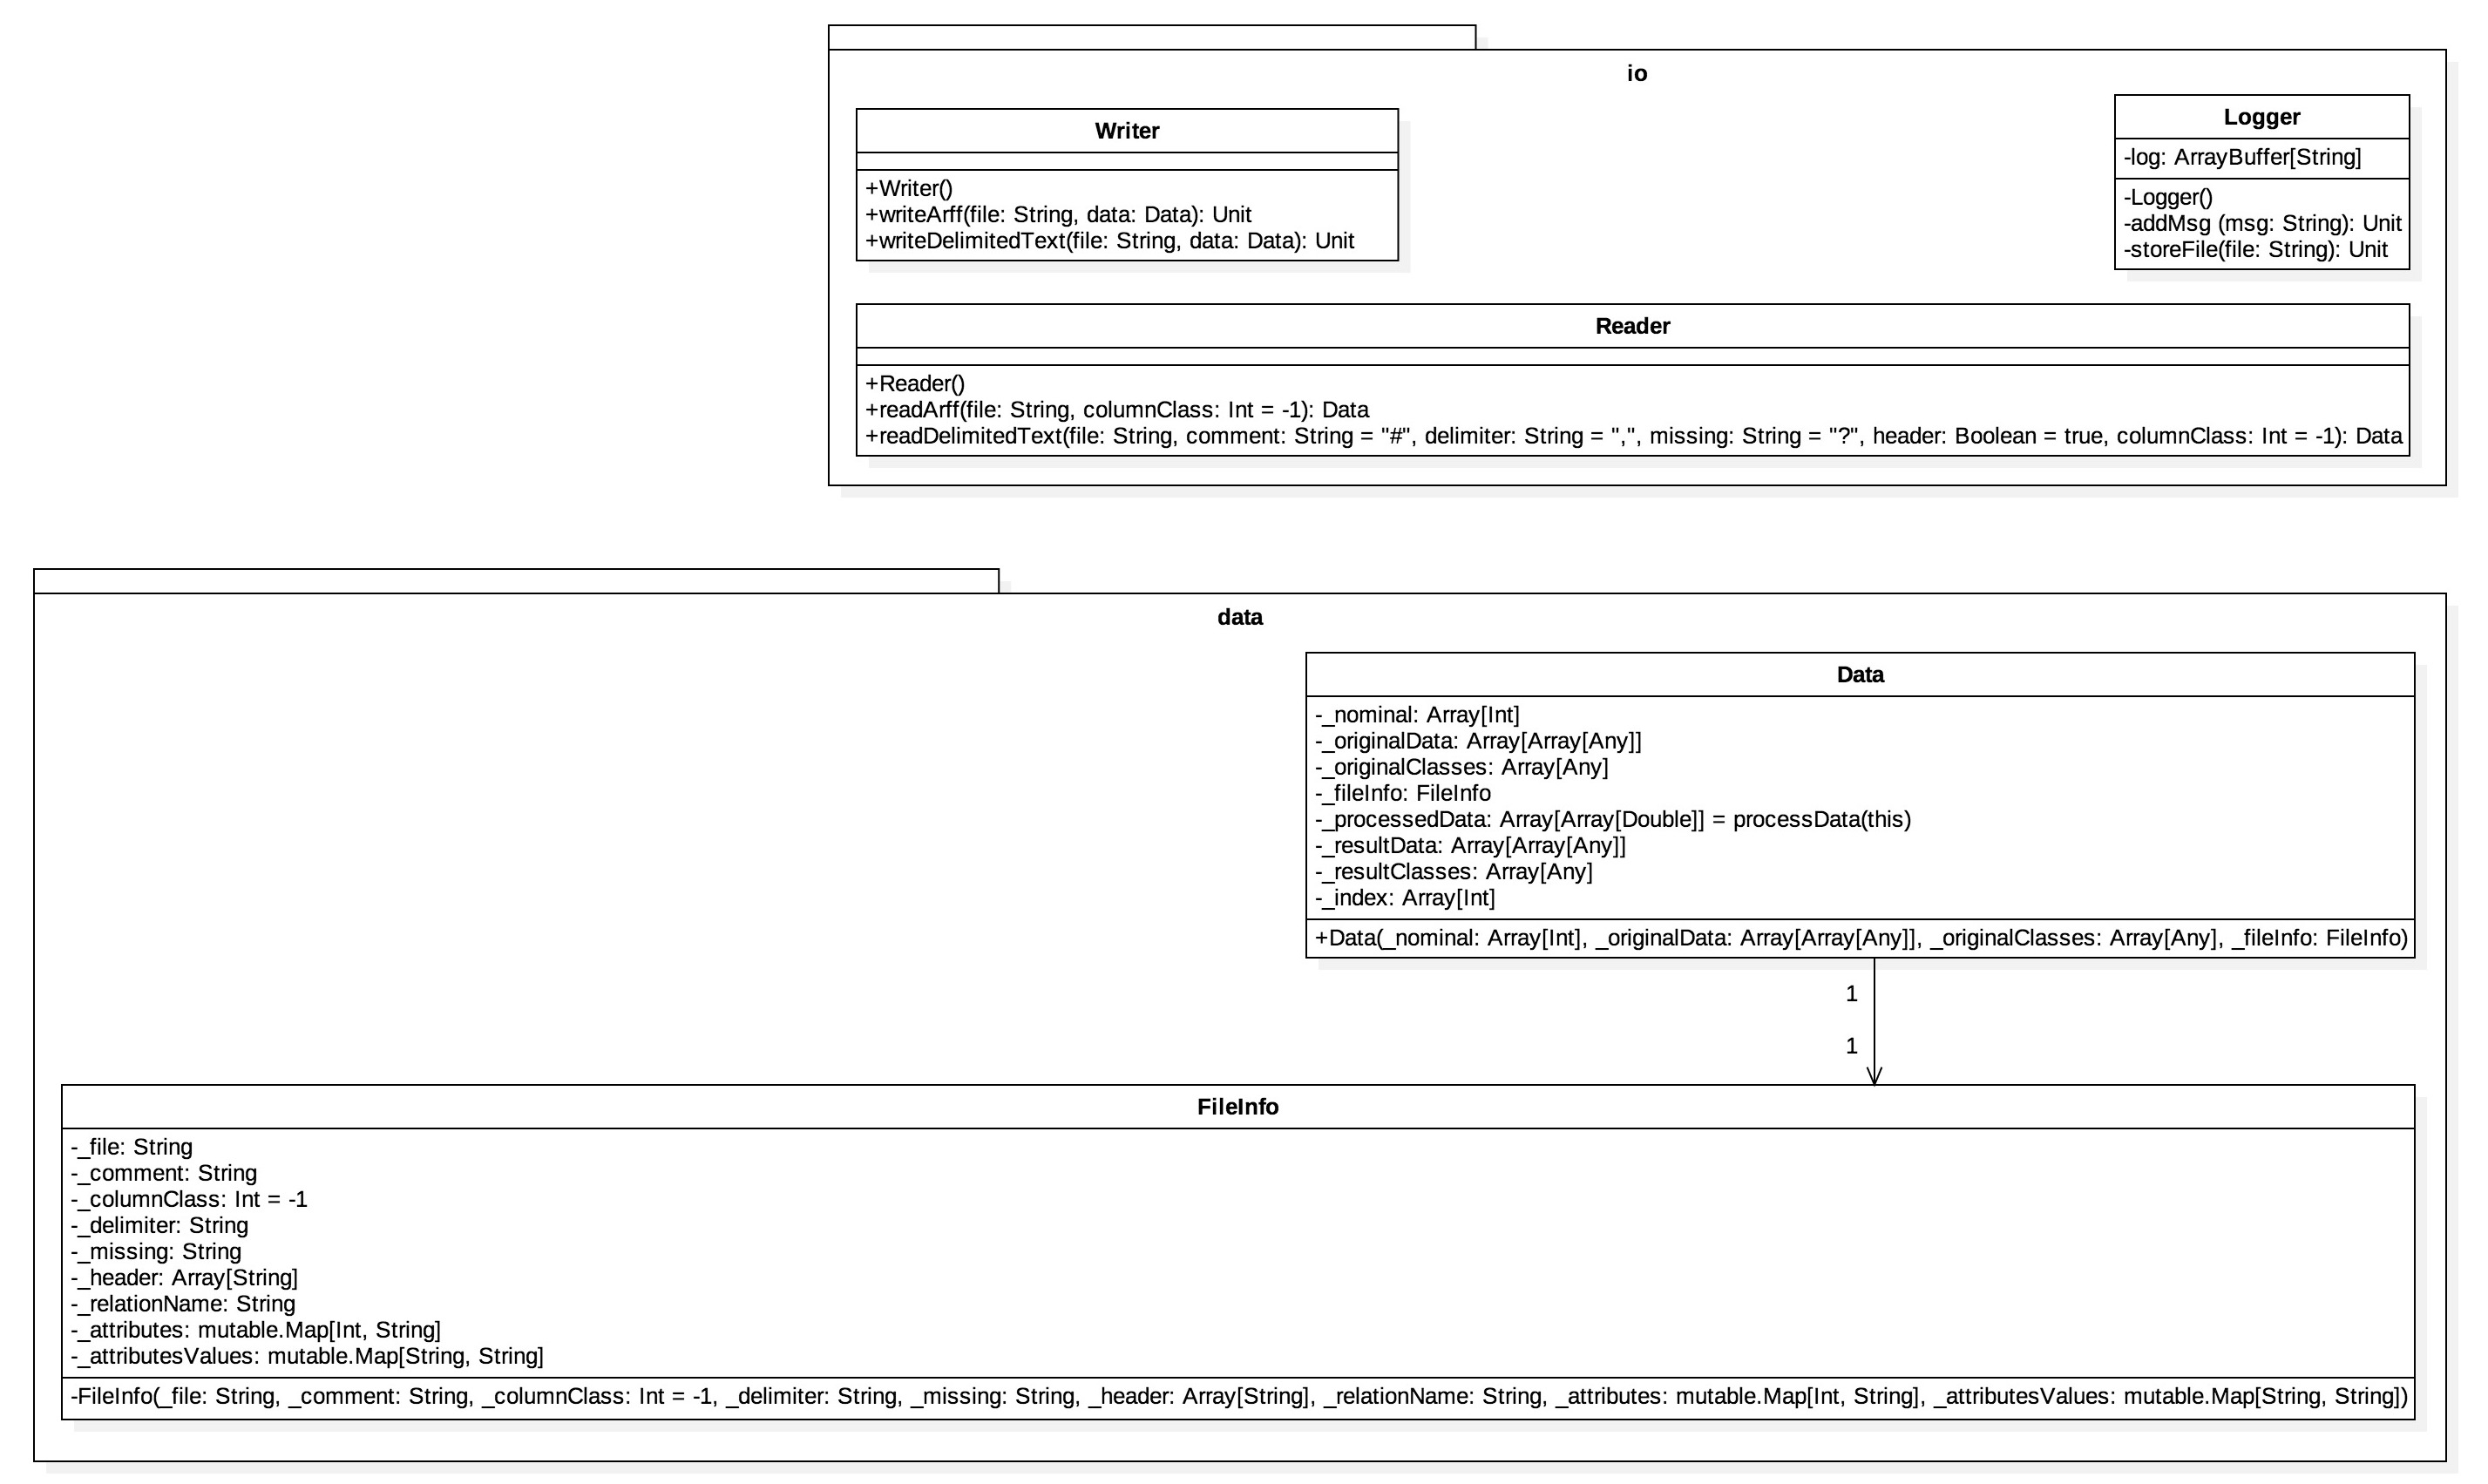
\includegraphics[scale=0.2, angle=90]{./imagenes/3_clases_detalles_pt1.jpg}
\end{figure}

\begin{figure}[H]
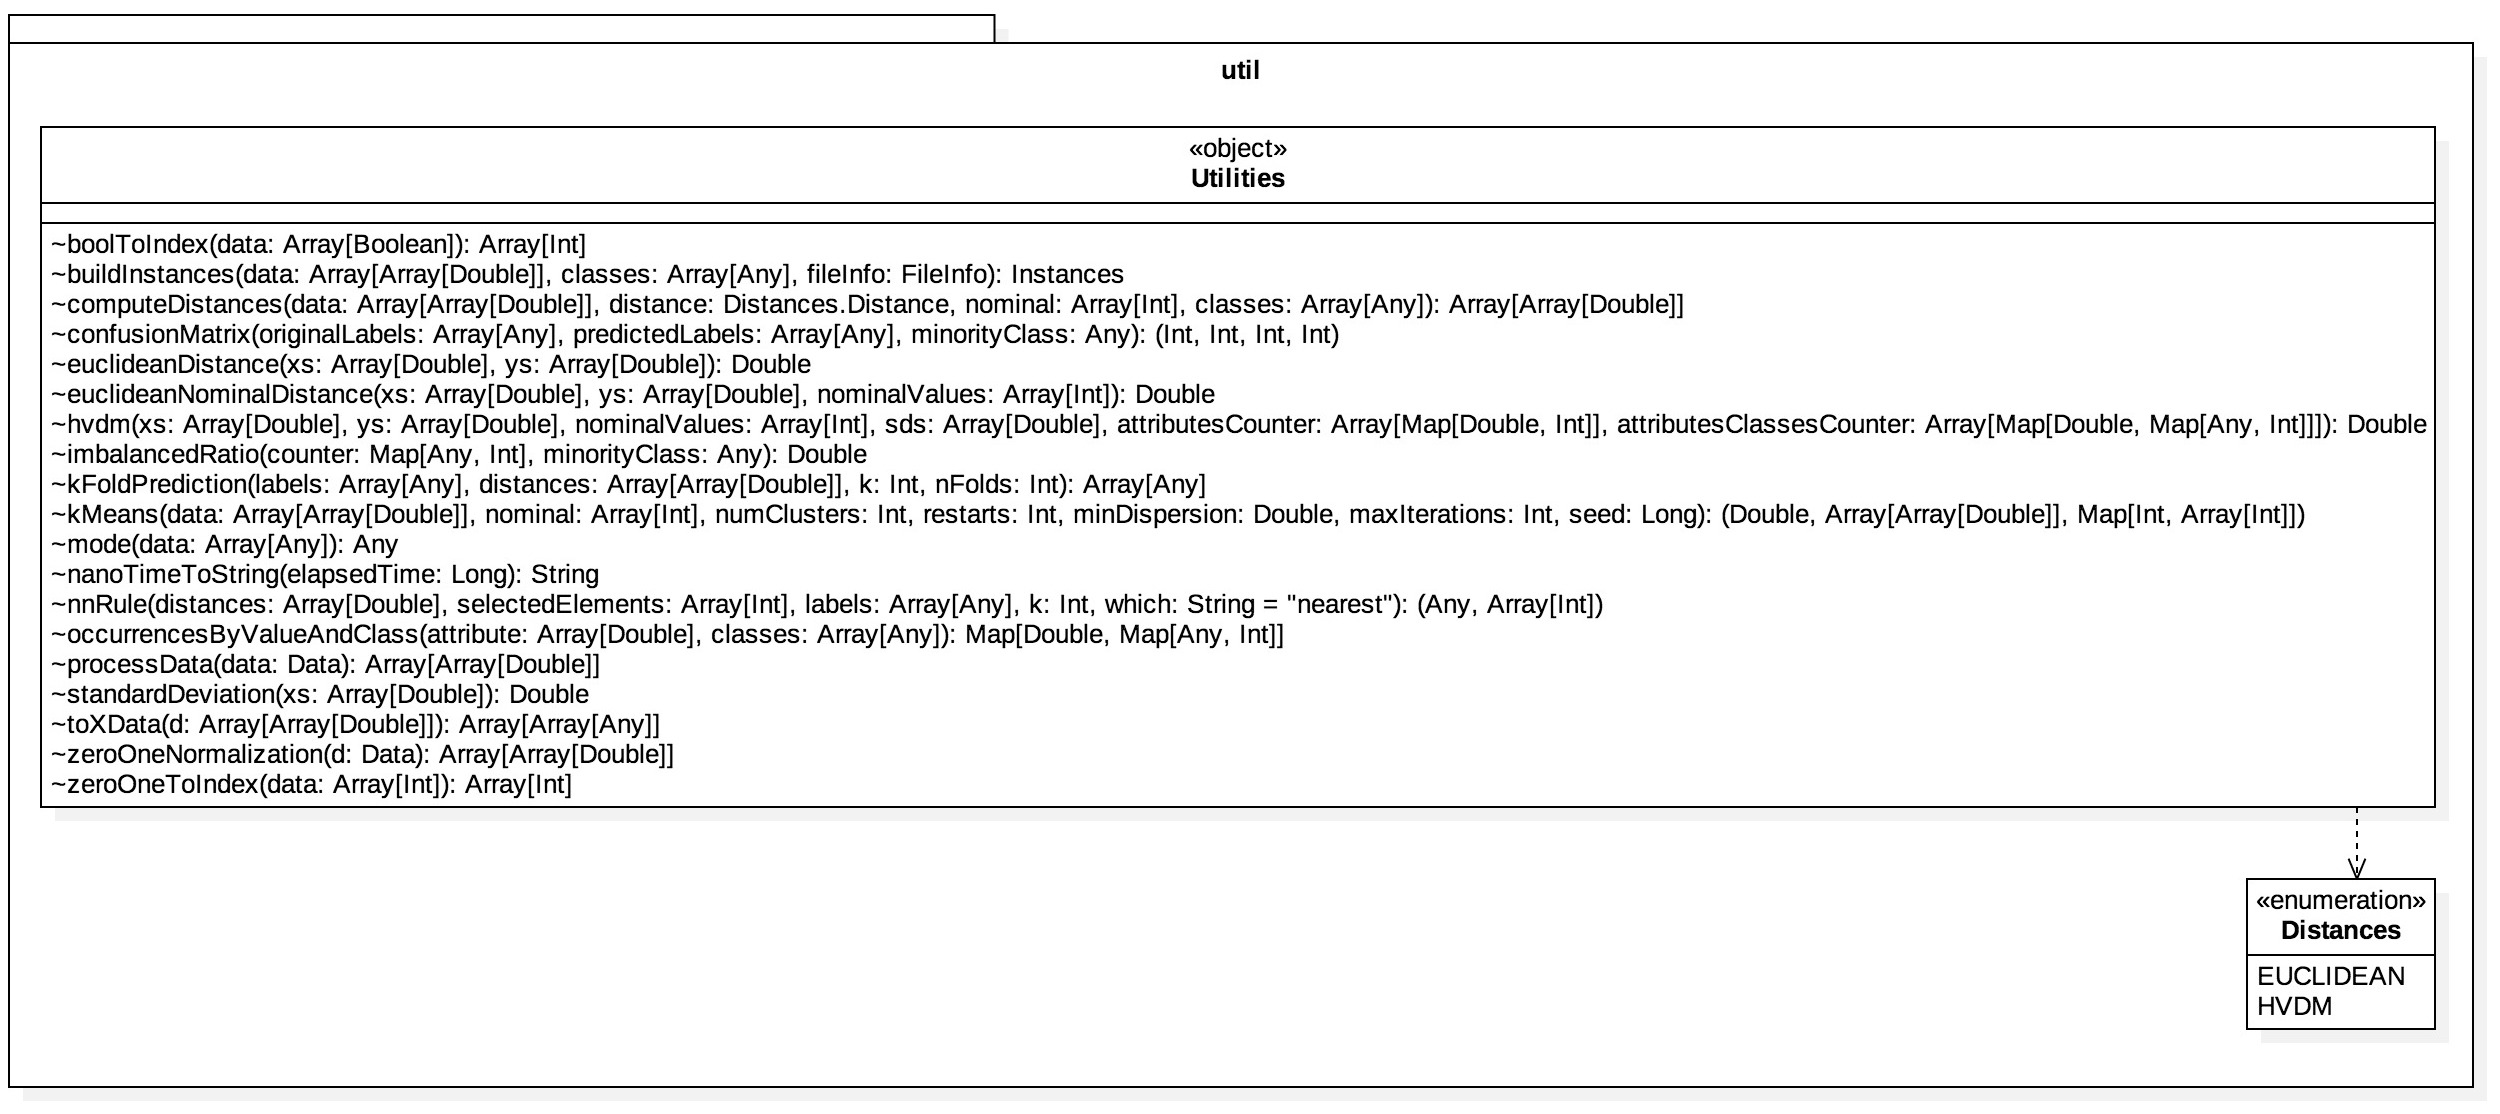
\includegraphics[scale=0.23, angle=90]{./imagenes/3_clases_detalles_pt2.jpg}
\end{figure}

\begin{figure}[H]
\centering
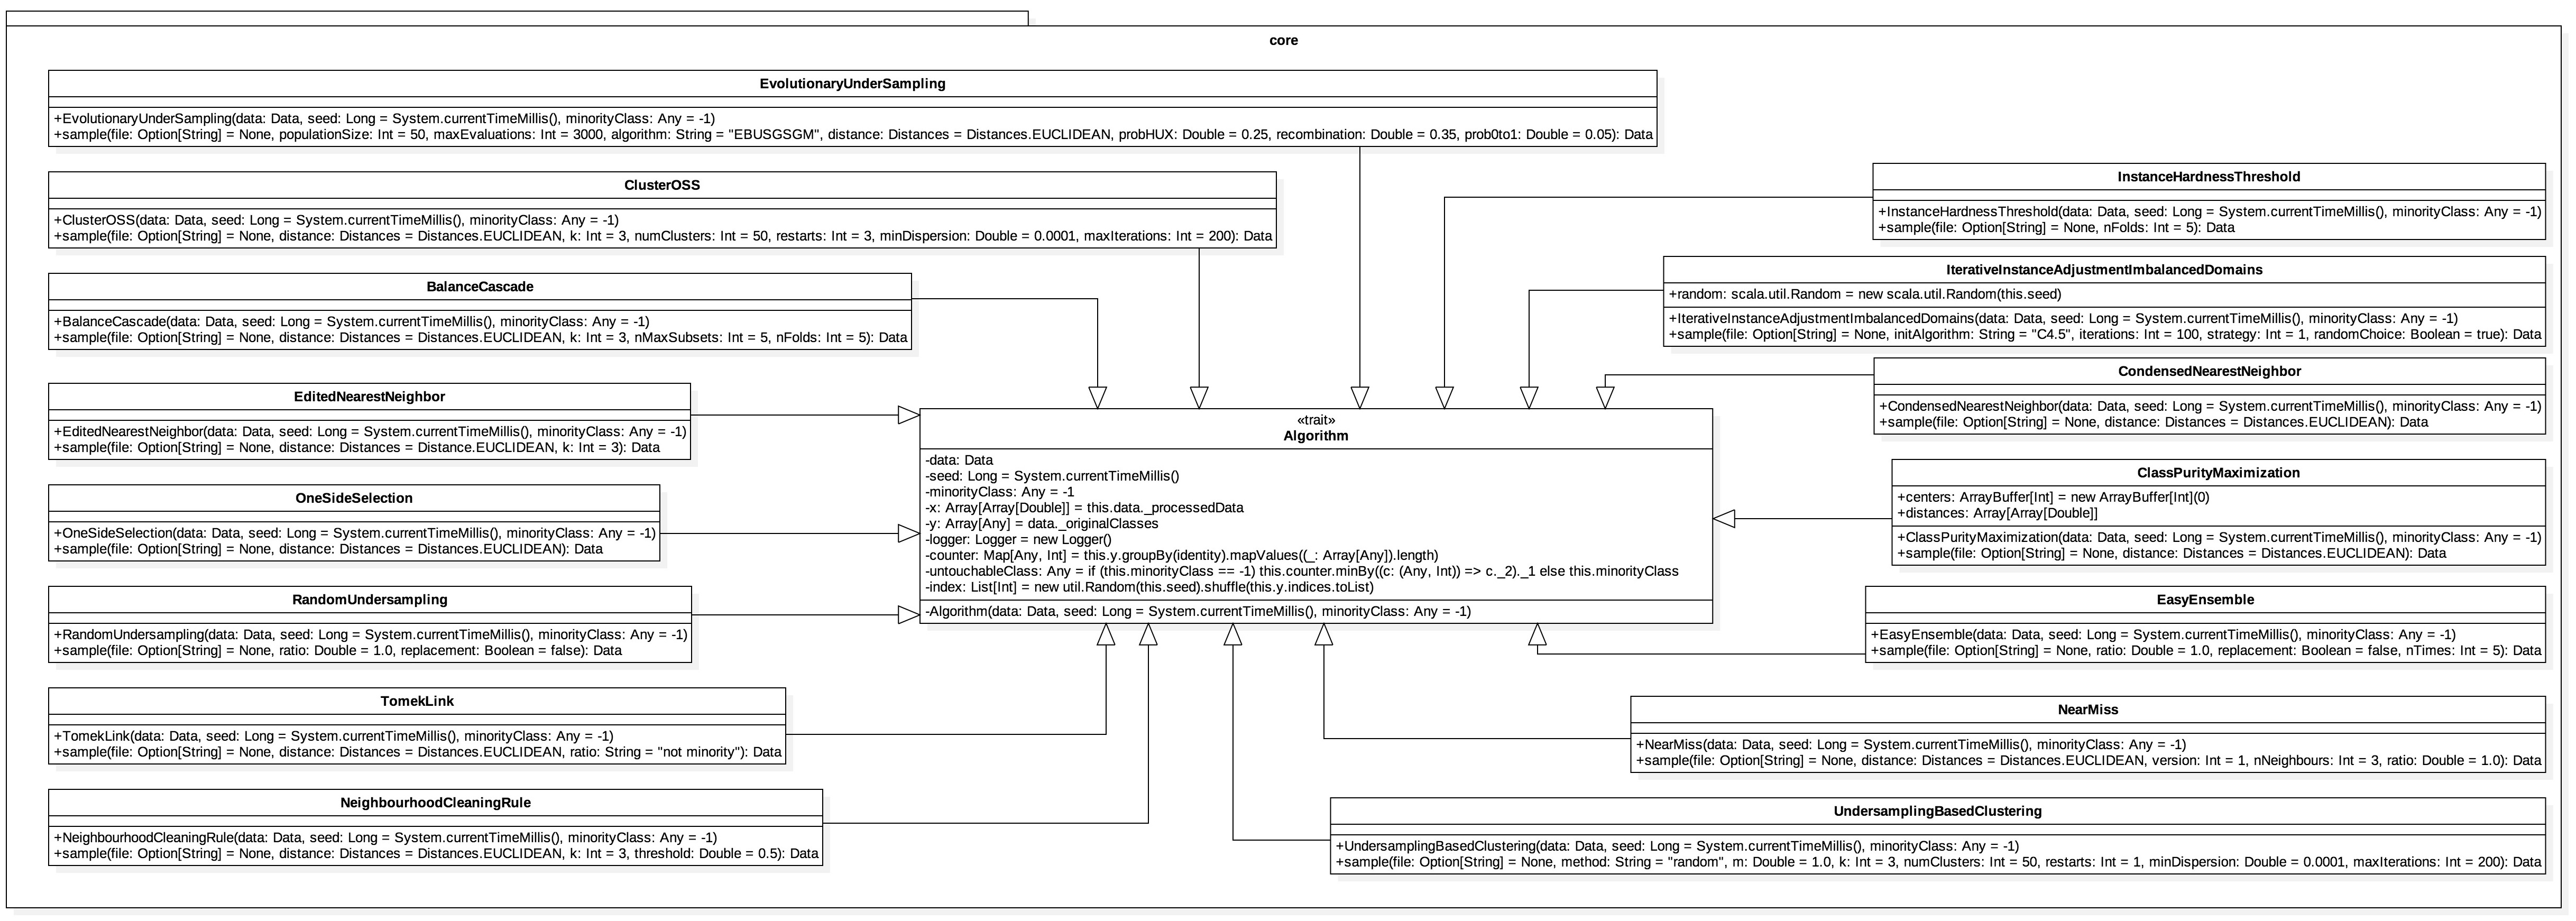
\includegraphics[scale=0.13, angle=90]{./imagenes/3_clases_detalles_pt3.jpg}
\end{figure}

\section{Presupuesto.} \label{sec:presupuesto}

Para la implementación de este proyecto se hubiese necesitado un presupuesto más o menos básico:

\begin{itemize}
	\item \textit{Un ordenador para desarrollo:} en mi caso se ha utilizado un \textit{MacBook Pro} del fabricante \textit{Apple} valorado en \textit{3300 euros}. Este es mi ordenador personal y por eso lo he usado, pero no sería necesario un ordenador tan potente. Un ordenador con un sistema \textit{Unix} y un procesador medianamente en condiciones hubiese sido suficiente, reduciendo el coste a unos \textit{800-1000 euros}.
	\item \textit{Conexión a Internet:} recurso indispensable para acceder a la documentación de \textit{Scala} y los \textit{papers} de los artículos. Dado que no se hacen grandes transferencias de datos, tampoco es necesario una conexión de gran velocidad. En mi caso se ha usado una conexión de fibra óptima de \textit{50Mb} con un precio de unos \textit{30 euros} al mes.
	\item \textit{Suministro eléctrico:} necesario para poder alimentar el ordenador. Dado que se trata de una biblioteca que maneja grande volúmenes de datos se hace un uso intenso del procesador, lo cual supone un alto consumo de batería y por tanto eléctrico.
	\item \textit{Salario:} estimo haber echado unas 350 horas en realizar todo el proyecto, incluyendo todas las partes del mismo. Supongamos que se pagan a diez euros la hora, el dinero necesario rondaría los tres mil quinientos euros.
\end{itemize}

\section{Requisitos funcionales.} \label{sec:requisitos}

Para que se trate de una biblioteca competitiva debe cumplir los siguiente requisitos:

\begin{itemize}
	\item \textit{Alta velocidad de procesamiento:} se trata de una biblioteca que puede manejar grandes volúmenes de datos. Si para conjuntos pequeños el tiempo de ejecución es elevado, este será enorme cuando se introduzca mayor volumen de datos.
	\item \textit{Diferentes formatos de entrada:} hoy en día los datos pueden venir de distintos origines y, por lo tanto, debemos estar preparados para leer una gran variedad de formatos. Esta biblioteca es capaz de leer datos en formato \textit{ARFF} \cite{arffwiki} de \textit{Weka} \cite{weka} \cite{wekaweb} y datos en cualquier formato de texto plano indicando los tokens necesarios, como puede ser el separados de elementos, el token de comentario, el token que representa valores nulos, \textit{etcetera}.
	\item \textit{Diferentes formatos de salida:} al igual que sucede con la entrada de datos, sucede con los datos de salida. Esta biblioteca permite los mismos formatos de salida que de entrada, facilitando así al usuario la posibilidad de tener el resultado de los algoritmos en el mismo formato de entrada —u otro a elegir—.
	\item \textit{Seguro a errores:} este tipo de algoritmos tiene una gran variedad de parámetros y, por lo tanto, distintas configuraciones que el usuario puede elegir. Todos los algoritmos están probados con distintos valores de estos parámetros y los propios algoritmos comprueban que los argumentos son válidos. 
	\item \textit{Datos intactos:} los datos de entrada son modificados en la mayoría de los algoritmos para poder trabajar con ellos, pero no nos podemos permitir devolver los datos modificados, ya que esos no son los datos que ha introducido el usuario. Para evitar esto, todos los algoritmos —con excepción del algoritmo \textit{IPADE-ID} ya que crea nuevos datos sintéticos y, por lo tanto, no es posible garantizar esta condición— trabajan con índices a los datos en vez de con los propios datos, para así no poder devolver los datos originales accediendo a las posiciones indicadas por el índice. Esto también nos proporciona una mayor velocidad de procesamiento, ya que es más eficiente trabajar con una colección de índices que con una matriz de \textit{n $\times$ m} elementos.
\end{itemize}